\documentclass[a4paper,11pt]{article}

\renewcommand\bottomfraction{0.9} % default value: 0.3
\renewcommand\textfraction{0.1}   % default value: 0.2

\usepackage{caption}
\usepackage{array}
\usepackage{fullpage, setspace, url}
\usepackage{colortbl}
\usepackage{amsmath}
\usepackage{indentfirst}
%\usepackage{algorithm,algorithmic}
%\definecolor{G6}{rgb}{0.7,0.7,0.7}
%\newcommand{\fc}{\cellcolor{G6}}
\usepackage{subfigure}
\usepackage{multirow}
\usepackage[table]{xcolor}
\usepackage{graphicx} 
\usepackage{bmpsize}
\usepackage{pgfgantt}

% pacotes malucões
\usepackage{graphicx}
\usepackage{amsfonts}
\usepackage{amssymb}
\usepackage{amstext}
\usepackage{hyperref}
\usepackage{ragged2e}
\usepackage{color}
\usepackage{enumerate}
\usepackage{float}
% fonte
\usepackage{helvet}
% coisas de locale
\usepackage[brazil]{babel}
\usepackage[utf8]{inputenc}
\usepackage[T1]{fontenc}
\usepackage{tabularx}

\addtolength{\textwidth}{2cm}
\addtolength{\hoffset}{-1cm}

\addtolength{\textheight}{2cm}
\addtolength{\voffset}{-1cm}

\newcommand{\HRule}{\rule{\linewidth}{0.5mm}}
\newcommand{\DUVIDA}[1]{\huge \textbf {\color{red} #1}\normalsize \\} % escreve uma dúvida grandão vermelha

\begin{document}
% \maketitle

\begin{center}
    \pagestyle{empty} 
    % Upper part of the page
    \textsc{\Large Universidade de São Paulo\\
    Instituto de Ciências Matemáticas e de Computação\\
    SSC0130 - Engenharia de Software - Turma A}\\[5.0cm]

    % Title
    \HRule \\[0.6cm]
    {\Huge Projeto parte 2\\
    Plano de Projeto}\\[0.4cm]
    \HRule \\[3.5cm]

    % Author and supervisor
    \begin{minipage}{0.45\textwidth}
	    \begin{flushleft} \normalsize
    		\emph{Alunos:}
    		
			\[\begin{array}{lr}
	    		\text{Gil Barbosa Reis} & 8532248 \\
    			\text{Giovane Cunha Mocellin} & 8578382 \\
		    	\text{Leonardo Sampaio Ferraz Ribeiro} & 8532300 \\
				\text{Rogério P. Souza} & 5626341
    		\end{array}\]
    	\end{flushleft}
    \end{minipage}
    \begin{minipage}{0.45\textwidth}
	    \begin{flushright} \normalsize
    		\emph{Professora:} \\
    		Ellen Francine Barbosa
	    \end{flushright}
    \end{minipage}

    \vspace{3.0cm}


    \vfill
    % Bottom of the page
    {\Large São Carlos, SP \\ \today}
    \thispagestyle{empty} 
    \newpage
\end{center}

\pagestyle{plain}
\setcounter{page}{1}
\setstretch{1.2}
\newpage

\tableofcontents
\listoffigures
\listoftables
\newpage

\section{Introdução}
	\subsection{Objetivo do projeto}
		O objetivo deste documento é, entre outros, estabelecer o escopo do projeto, determinar sua viabilidade, analisar os riscos associados, definir recursos necessários, estimar custos e esforço e desenvolver um cronograma do projeto.

	\subsection{Escopo do projeto}
		\subsubsection{Descrição do produto}
			O T-play é  um site voltado para a troca e venda de jogos, tanto físicos, como digitais.
			Os usuários comuns poderão utilizar o sistema para cadastrar ofertas de seus jogos, efetuar a troca de jogos com outros usuários e 
pesquisar ofertas de seu interesse.
			Durante a transação (troca ou venda) entre usuários, pode haver troca de mensagens entre ambos.
			Ao final das transações, usuários devem atribuir uma nota ao outro usuário participante, e uma nota à usabilidade do T-play.
			Há um sistema de ranqueamento que ajuda o usuário durante a escolha do melhor candidato à troca.
			Além disso, caso o usuário queira ofertar um jogo que não exista no sistema, o mesmo pode sugerir o cadastro de tal jogo.
			
			Os administradores poderão utilizar o sistema para gerenciar os patrocinadores e outros administradores, moderar negociações problemáticas, gerenciar cadastro de novos jogos e acessar os diversos relatórios.

			Os patrocinadores possuem os mesmos direitos e restrições que os usuários comuns, mas também recebem, mediante a pagamento em interface exclusiva, o direito de apresentar propagandas no site que redirecionam e enfatizam seus oferecimentos de jogos.

		\subsubsection{Principais entregas do projeto}
			\begin{itemize}
				\item Documento de Requisitos
				\item Plano de projeto (este documento)
				\item Diagrama WBS
				\item Rede PERT com caminho crítico
				\item Tabela de alocação de recursos
				\item Gráfico de Gannt
			\end{itemize}

		\subsubsection{Objetivos do projeto}
			O objetivo do projeto é reduzir o esforço e tempo gastos atualmente por pessoas que trocam jogos pela internet e são obrigados a usarem outros meios de comunicação não destinados a esse fim.
		\newpage
		\subsubsection{Critérios de aceitação do produto}
			\begin{itemize}
				\item Ter menos de 5\% de avaliações negativas sobre a usabilidade do sistema em transações
				\item Responder a consultas em no máximo 5 segundos.
				\item Imprimir relatórios em no máximo 20 segundos.
				\item Ter no máximo 15 minutos de downtime/mês
				\item Um usuário qualquer deve conseguir sair de qualquer página do sistema e efetuar uma transação em menos de 3 cliques.
			\end{itemize}
	
\section{Cronograma de Projeto}
	\subsection{WBS}
    	O WBS está representado na figura \ref{WBS}, incluída no final deste documento.
	\subsection{Rede PERT com Caminho Crítico}
		A Rede PERT-CPM está representado na figura \ref{PERT}, incluída no final deste documento.
	\subsection{Gráfico de Gannt}
		O Gráfico de Gannt está representado na figura \ref{gannt}, incluída no final deste documento.
	\subsection{Tabela de Alocação de Recursos}
	\begin{center}
	\begin{table}[H]
		\begin{tabularx}{\textwidth}{c|X|c|X|c}
			\textbf{Ativ.} & \textbf{Descrição} & \textbf{Precedência} & \textbf{Recursos} & \textbf{Duração(dias)} \\
			\hline
			T1 & Projetar Entrevista & Não tem & Pessoas & 1\\ \hline
			T2 & Entrevistar Usuário & 1 & Pessoas, Cliente & 3\\ \hline
			T3 & Brainstorm & 1 & Pessoas & 1\\ \hline
			T4 & Produzir documento de requisitos & 2, 3& Pessoas & 5\\ \hline
			T5 & Validar documento & 4 & Pessoas, Cliente & 2\\ \hline
			T6 & Elaboração do modelo conceitual& 5 & Ferramenta case UML & 4\\ \hline
			T7 & Casos de uso & 5 & Ferramenta Case UML & 5 \\ \hline
			T8 & Elaboração do protótipo V1& 5 & Designer, Ferramenta de prototipação & 5 \\ \hline
			T9 & Elaboração de DSS & 7 & Ferramenta case UML& 5\\ \hline
			T10 & Elaboração de contratos de operação& 9 & Pessoas & 3 \\ \hline
			T11 & Projetar modularização & 9 & Arquiteto de Software, Ferramenta case UML & 7\\ \hline
			T12 & Diagramas de comunicação & 10 & Ferramenta case UML & 10\\ \hline
			T13 & Validar projeto & 11 & Pessoas, Cliente & 1\\ \hline
			T14 & Teste de usabilidade com V1 & 8 & Pessoas & 3 \\ \hline
			T15 & Validar modelos & 12 & Pessoas, Cliente & 2 \\ \hline
			T16 & Pojeto do diagrama de classes & 13 & Ferramenta case UML & 7\\ \hline
			T17 & Projeto conceitual com MER & 13, 15 & Analista de banco de dados & 3 \\ \hline
			T18 & Alterações e validação do protótipo & 14 & Designer, Cliente, Pessoas & 2\\ \hline
			T19 & Projeto lógico relacional & 17 & Analista de banco de dados & 2 \\ \hline
			T20 & Projeto físico & 19 & Analista do banco de dados & 4\\ \hline
			T21 & Implementação do projeto OO & 16, 20 & Desenvolvedores & 30 \\ \hline
			T22 & Implementação do projeto físico de BD& 20 & Analista de banco de dados & 10\\ \hline
			T23 & Implementação das interfaces & 18 & Desenvolvedores & 20\\ \hline
			T24 & Integração do sistema& 21, 22, 23 & Desenvolvedores & 10\\ \hline
			T25 & Teste de unidade & 24 & Tester & 5 \\ \hline
			T26 & Teste de banco de dados & 24 & Tester & 3 \\ \hline
			T27 & Teste de integração & 24 & Tester & 5\\ \hline
			T28 & Teste de aceitação& 25, 26, 27 & Tester, Cliente & 2\\ \hline
			T29 & Elaborar manual & 28 & Pessoas & 4\\ \hline
			T30 & Treinamento dos administradores & 29 & Pessoas & 3\\ \hline
		\end{tabularx}
		\caption{Lista de Atividades / Precedência / Recursos e Duração}
	\end{table}
	\end{center}
	
\section{Matriz de Riscos}
	
	\begin{table}[H]
		\begin{tabular}{c|l|c|c|c}
			\textbf{ID} & \multicolumn{1}{c|}{\textbf{Risco}} & \textbf{Categoria} & \textbf{Prob.(\%)} & \textbf{Impacto} \\
			\hline
			1 & Estimativa de tamanho baixa 				& Tamanho do Produto			& 60 & 2 \\
			2 & Número de usuários maior que esperado 		& Tamanho do Produto			& 40 & 3 \\
			3 & Prazo final apertado 						& Impacto no Negócio			& 30 & 3 \\
			4 & Falta de treinamento nas tecnologias usadas	& Recursos humanos				& 20 & 2 \\
			5 & Alta rotação de pessoal 					& Recursos humanos				& 60 & 2 \\
			6 & Ausência de participação do cliente			& Conformidade à especificação	& 15 & 4 \\
			7 & Cliente resistente a mudanças 				& Conformidade à especificação	& 30 & 2 \\
			8 & Hardware servidor fornecido inadequado		& Funcionamento do sistema		& 30 & 1 \\
		\end{tabular}
		\caption{Tabela de riscos\\Impactos: 1 - Crítico; 2 - Significativo; 3 - Marginal; 4 - Negligenciável}
	\end{table}

	\begin{center}
	\begin{table}[H]
		\begin{tabularx}{\textwidth}{l|X|X|X|X|}
										& Negligenciável		& Mariginal				& Significativo			& Crítico \\ \hline
			Frequente (75$\sim$100\%) 	& \cellcolor{yellow}	& \cellcolor{red}		& \cellcolor{red}		& \cellcolor{red} \\ \hline
			Provável (50$\sim$75\%)		&						& \cellcolor{yellow}	& \cellcolor{red} 1, 5	& \cellcolor{red} \\ \hline
			Ocasional (25$\sim$50\%)	&  						& 2, 3					& \cellcolor{yellow} 7	& \cellcolor{red} 8 \\ \hline
			Improvável (0$\sim$25\%)	& 6						&						& 4						& \cellcolor{yellow} \\ \hline
		\end{tabularx}
		\caption{Matriz de riscos mapeados}
	\end{table}
	
	\end{center}
	\begin{table}[H]
		\begin{tabularx}{\textwidth}{c|X|X|X|X}
			\textbf{ID} & \multicolumn{1}{c|}{\textbf{Descrição}} & \multicolumn{1}{c|}{\textbf{Mitigação}} & \multicolumn{1}{c|}{\textbf{Resposta}} & \multicolumn{1}{c}{\textbf{Impacto}} \\
			\hline
			1 & Estimativa de tamanho baixa & Ter tolerância no cronograma & Estimar tempo acima para produção & Atraso na produção do sistema \\ \hline
			2 & Número de usuários maior que esperado & Considerar um servidor de capacidade elástica & Negociar com o cliente & Tempo de resposta prejudicado \\ \hline
			3 & Prazo final apertado & Aumentar o tempo de dedicação ao projeto & Pagar hora extra para os desenvolvedores envolvidos & Atraso na produção do sistema \\ \hline
			4 & Falta de treinamento nas tecnologias utilizadas & Ter pessoal treinado & Dar treinamento aos desenvolvedores envolvidos & Atraso na produção do sistema \\ \hline
			5 & Alta rotação de pessoal & Ter pessoal extra a par do projeto & Interar pessoal extra ao projeto & Atraso na produção do sistema \\ \hline
			6 & Ausência na participação do cliente & Ter maior comunicação com o cliente & Procurar o cliente mais & Produto incompatível com expectativas do cliente \\ \hline
			7 & Cliente resistente a mudanças & Comunicação com cliente & Negociar mudanças suaves com cliente & Atraso na produção do sistema \\ \hline
			8 & Hardware servidor fornecido inadequado & Ter um hardware adequado & Negociar o hardware oferecido com o cliente & Tempo de resposta prejudicado \\
		\end{tabularx}
		\caption{Tabela de mitigação de Riscos}
	\end{table}

\section{Conclusão}
	Considerando cinco desenvolvedores de software trabalhando 8 horas/dia, a rede PERT-CPM foi construída e, a partir da mesma, foi possível identificar que o tempo de  desenvolvimento ideal para o projeto é 99 dias úteis. Com base nesse tempo, e em uma média de pagamento de 15 reais/hora dos desenvolvedores, é estimado um custo de mão-de-obra de R\$59.400,00. Além do custo de mão-de-obra, estimam-se que serão gastos R\$1.000,00 nas licensas das ferramentas extras utilizadas (ferramenta Case UML e de prototipação).

		\begin{figure}[!H]
    		\centering
        	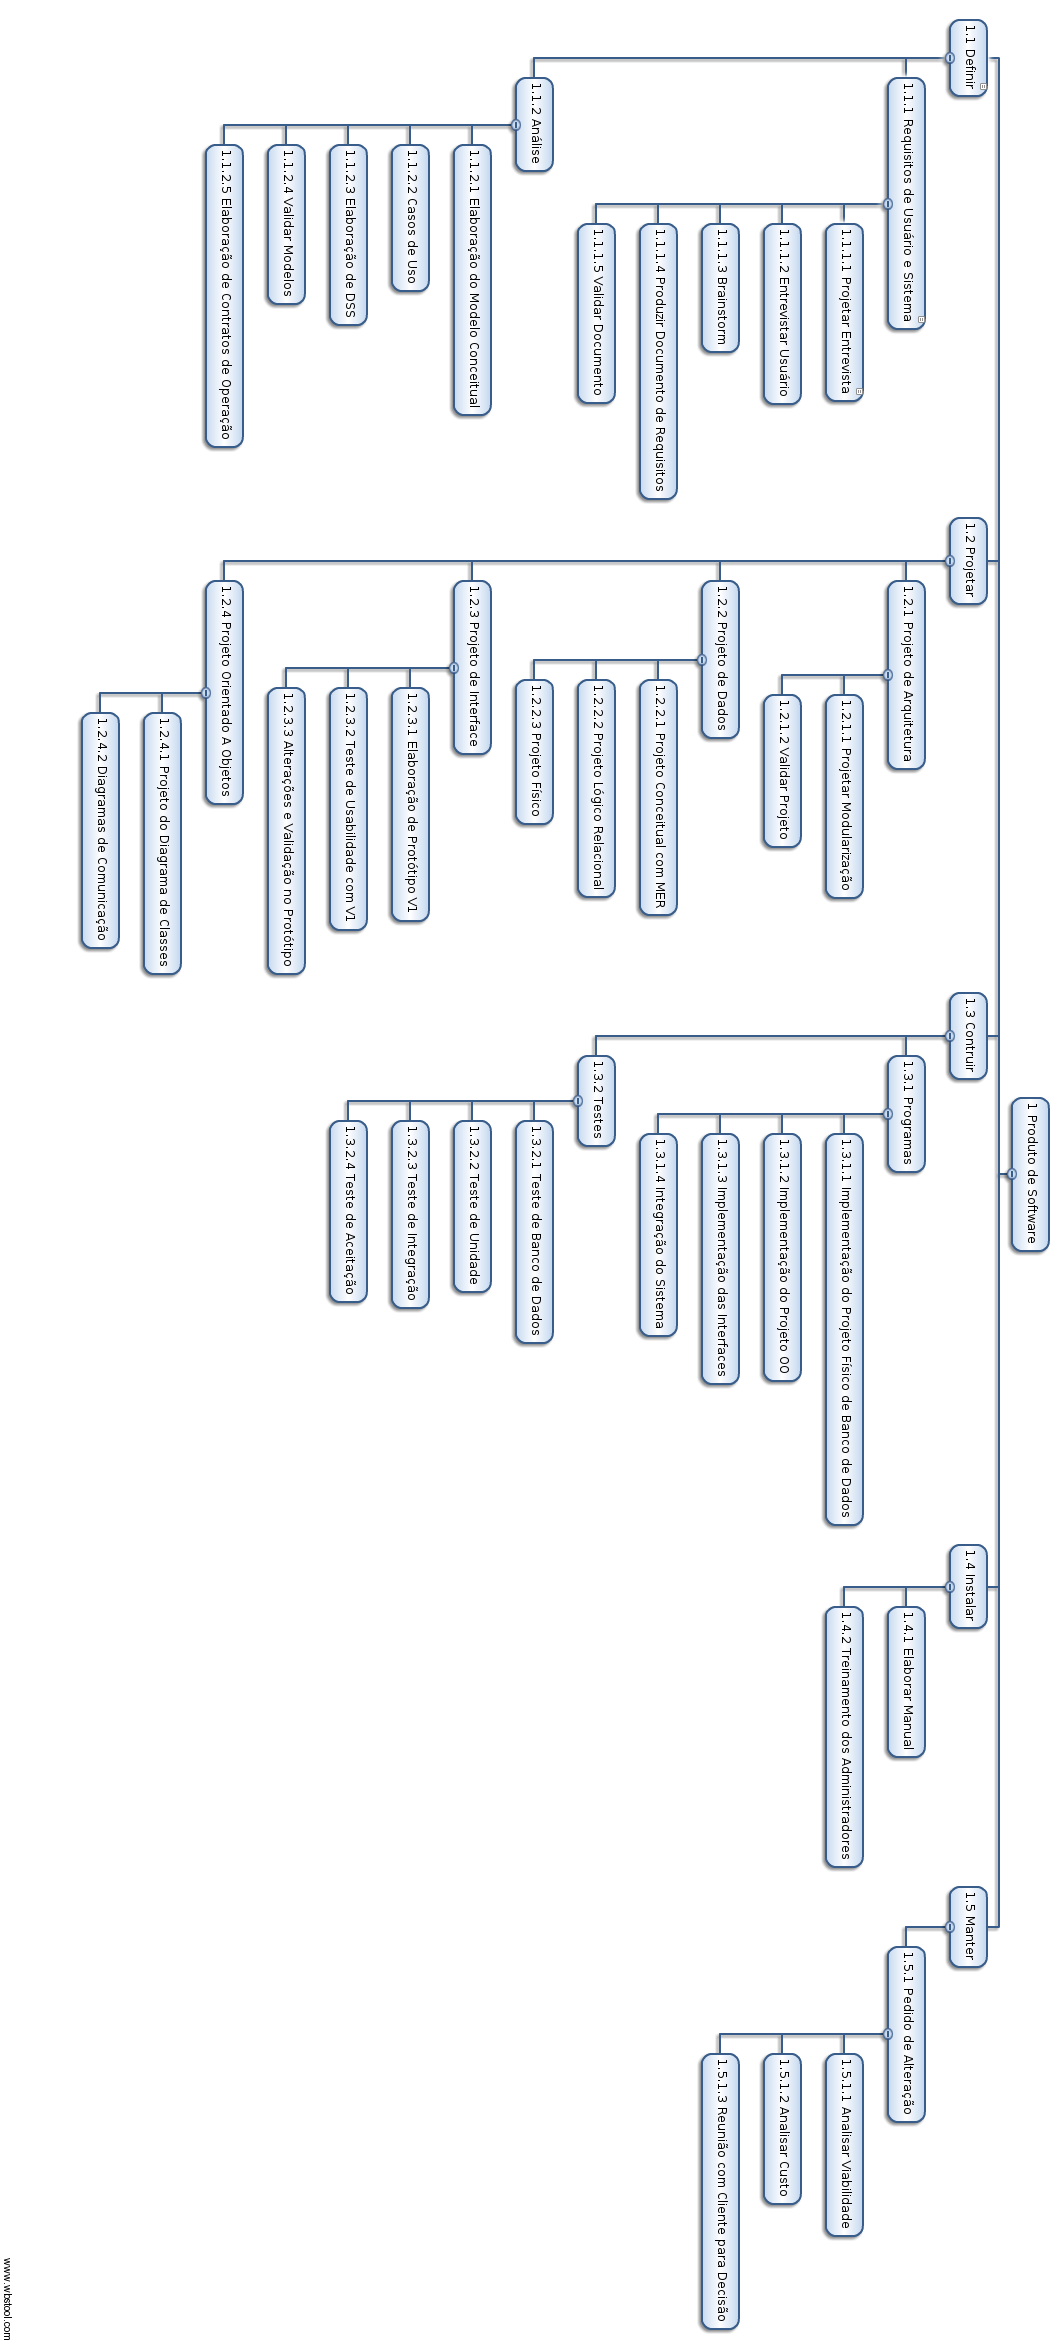
\includegraphics[width=\textwidth,height=\dimexpr\textheight-3\baselineskip\relax,keepaspectratio]{WBS.png}
        	\caption{WBS}
     		\label{WBS}
    	\end{figure}
    	\begin{figure}[!H]
    		\centering
        	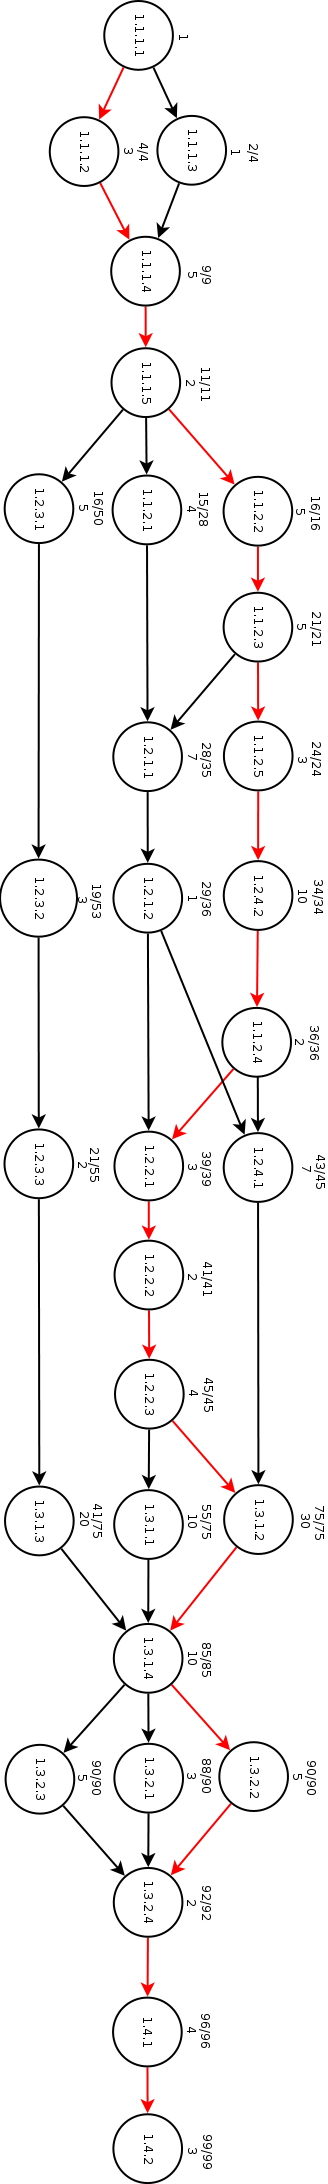
\includegraphics[width=\textwidth,height=\dimexpr\textheight-3\baselineskip\relax,keepaspectratio]{engsoft_pert2.png}
        	\caption{Rede PERT-CPM}
     		\label{PERT}
    	\end{figure}
    	\begin{figure}[!H]
    		\centering
        	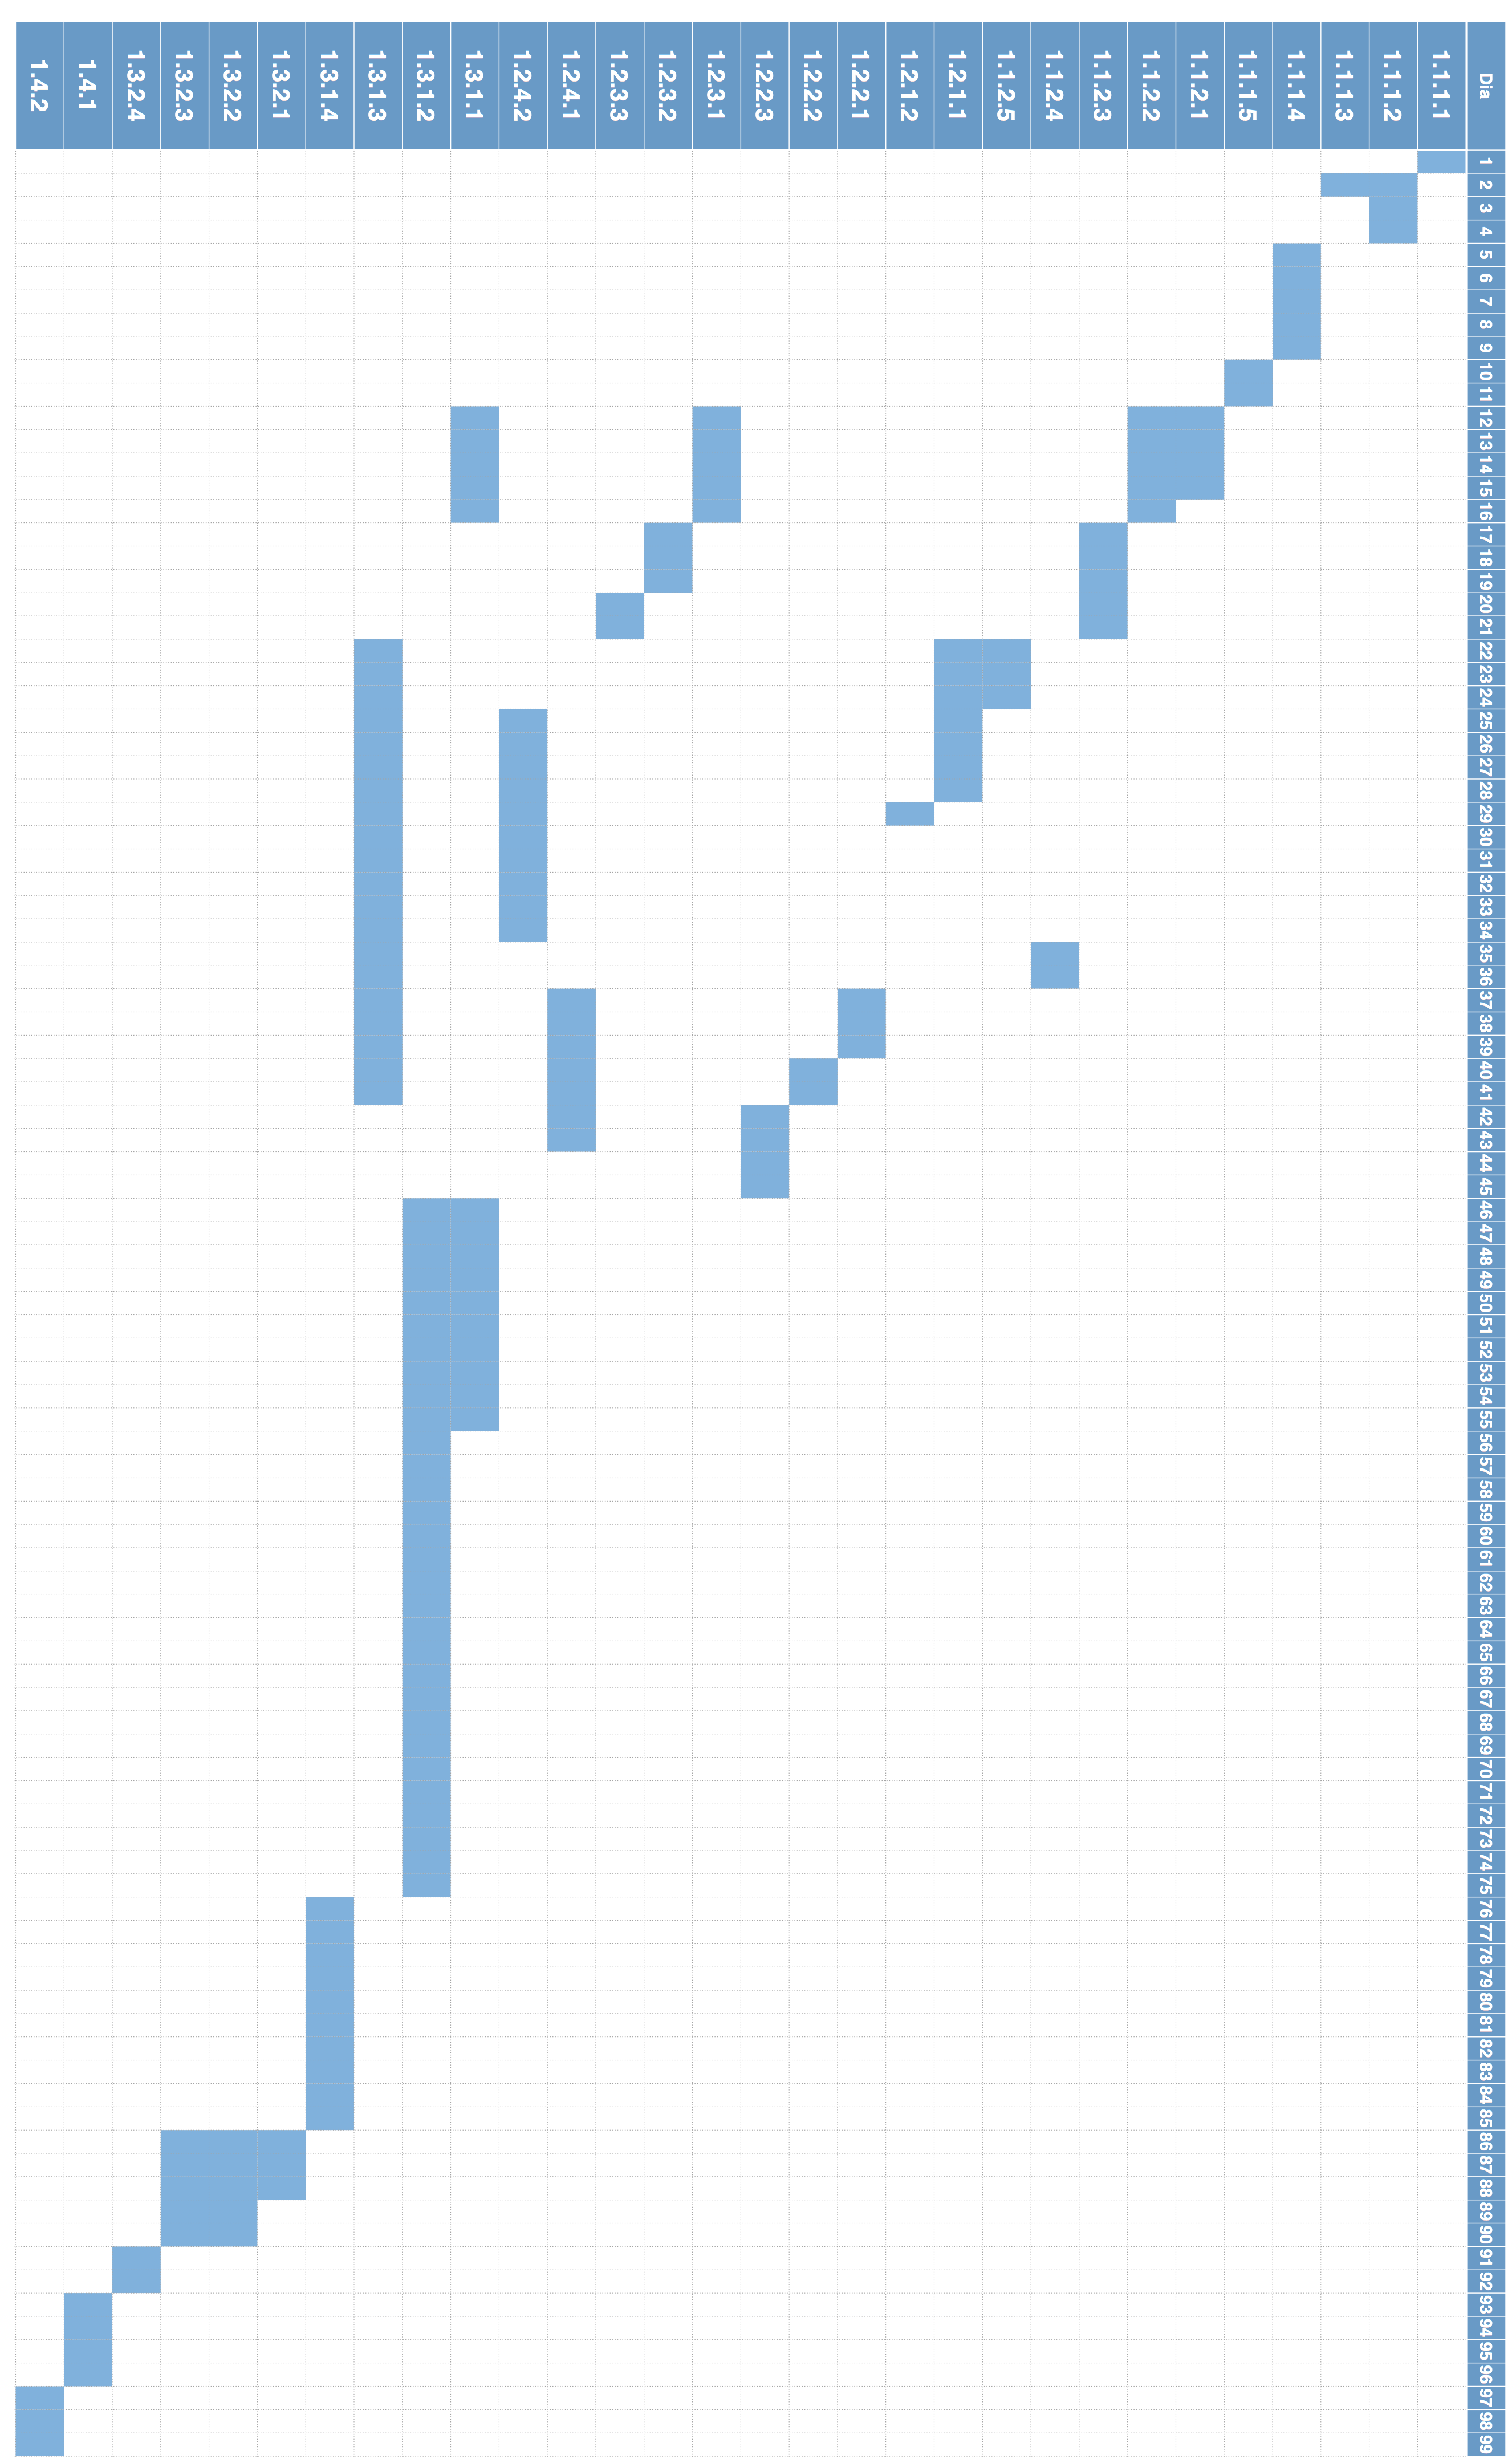
\includegraphics[width=\textwidth,height=\dimexpr\textheight-3\baselineskip\relax,keepaspectratio]{gannt.png}
        	\caption{Gráfico Gannt}
     		\label{gannt}
    	\end{figure}

\end{document}
